\begin{figure}[!t]
    \centering
    \subfigure{
        \begin{minipage}[t]{0.11\textwidth}
            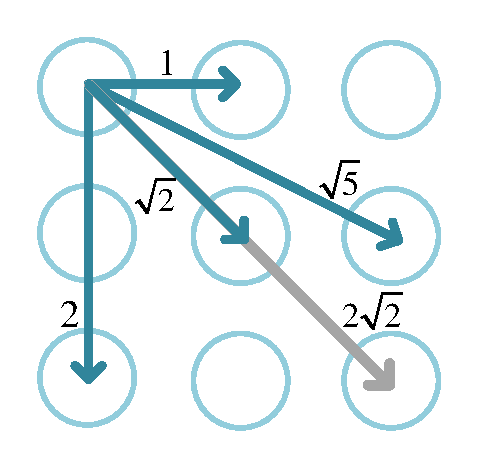
\includegraphics[width=\textwidth]{fig/physical_length.pdf}\\
            \centering \footnotesize (a) line length
        \end{minipage}
    }
    \hspace{0.1cm}
    \subfigure{
        \begin{minipage}[t]{0.11\textwidth}
            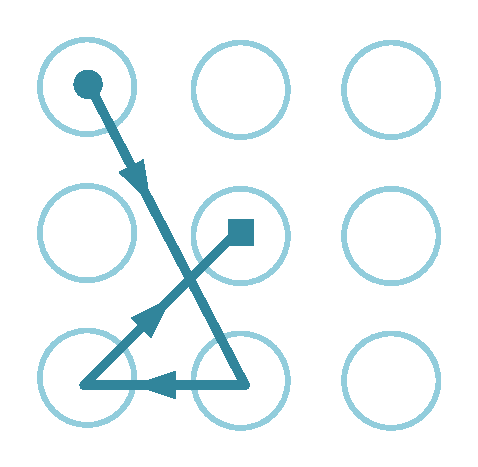
\includegraphics[width=\textwidth]{fig/intersection.pdf}\\
            \centering \footnotesize (b) line intersection
        \end{minipage}
    }
    \hspace{0.1cm}
    \subfigure{
        \begin{minipage}[t]{0.11\textwidth}
            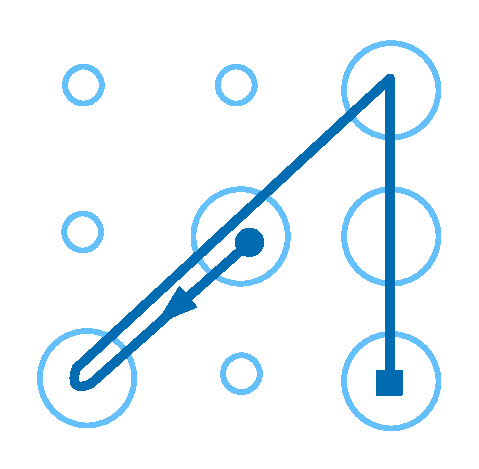
\includegraphics[width=\textwidth]{fig/overlap.pdf}\\
            \centering \footnotesize (c) overlapping lines
        \end{minipage}
    }
    \caption{Illustrations of the terminologies used in Equation~\ref{equ:compscore}.}
    \label{fig:intersection-overlap}
\end{figure}
\begin{figure}[!t]
            \centering
            \subfigure{
                \begin{minipage}[b]{8cm}
                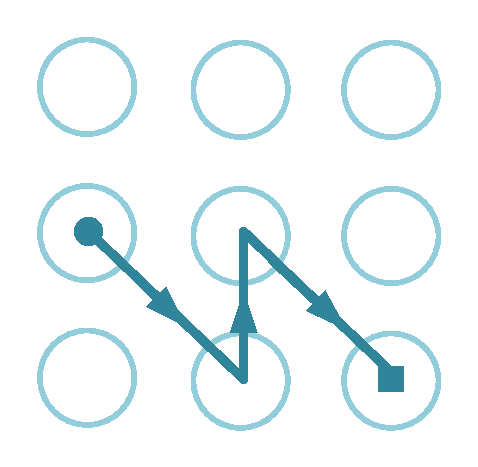
\includegraphics[width=1.3cm]{fig/9-1.pdf}
                \hspace{0.1cm}
                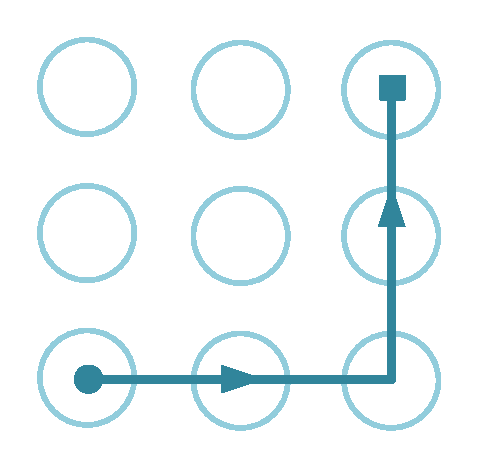
\includegraphics[width=1.3cm]{fig/9-2.pdf}
                \hspace{0.1cm}
                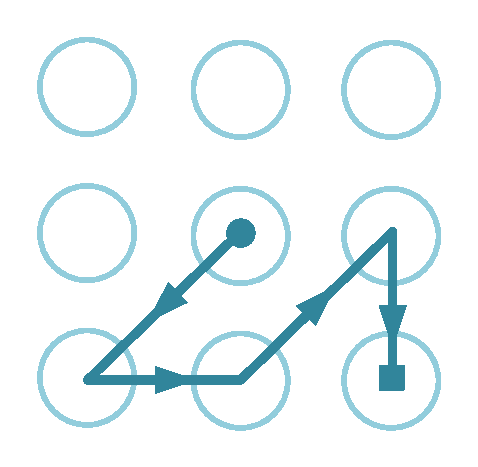
\includegraphics[width=1.3cm]{fig/9-3.pdf}
                \hspace{0.1cm}
                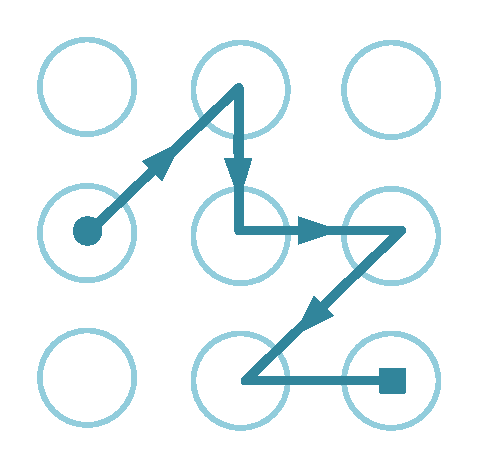
\includegraphics[width=1.3cm]{fig/9-4.pdf}
                \hspace{0.1cm}
                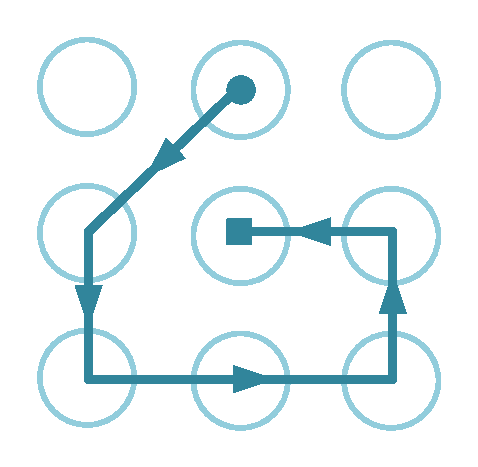
\includegraphics[width=1.3cm]{fig/9-5.pdf}\\
                \centering \footnotesize (a) Example patterns belong to the simple category.
                \end{minipage}
            }
            \subfigure{
                \begin{minipage}[b]{8cm}
                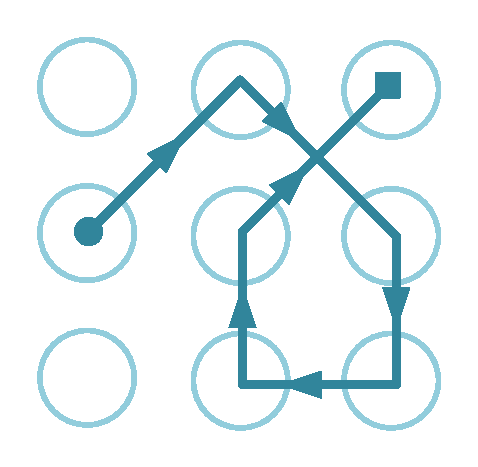
\includegraphics[width=1.3cm]{fig/9-6.pdf}
                \hspace{0.1cm}
                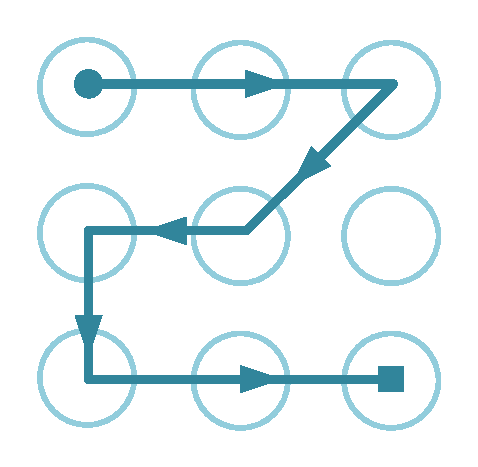
\includegraphics[width=1.3cm]{fig/9-7.pdf}
                \hspace{0.1cm}
                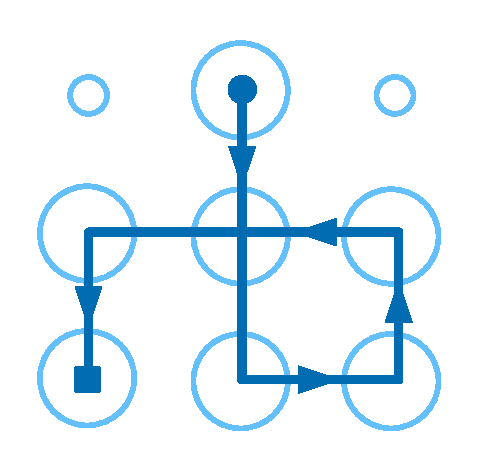
\includegraphics[width=1.3cm]{fig/9-8.pdf}
                \hspace{0.1cm}
                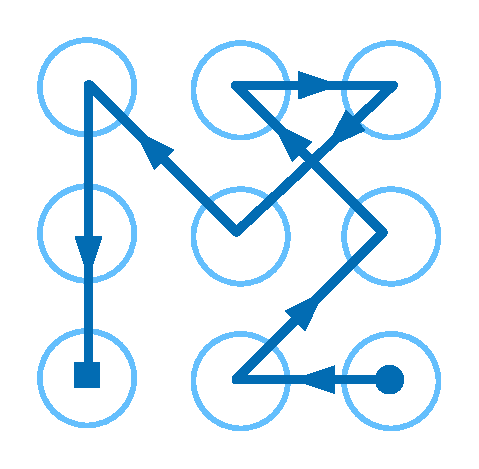
\includegraphics[width=1.3cm]{fig/9-9.pdf}
                \hspace{0.1cm}
                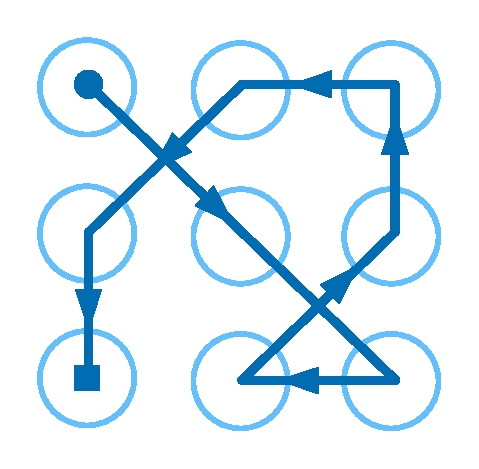
\includegraphics[width=1.3cm]{fig/9-10.pdf}\\
                \centering \footnotesize (b) Example patterns belong to the median category.
                \end{minipage}
            }
            \subfigure{
                \begin{minipage}[b]{8cm}
                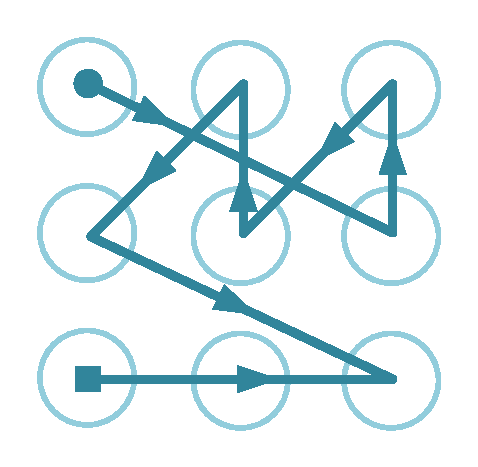
\includegraphics[width=1.3cm]{fig/9-11.pdf}
                \hspace{0.1cm}
                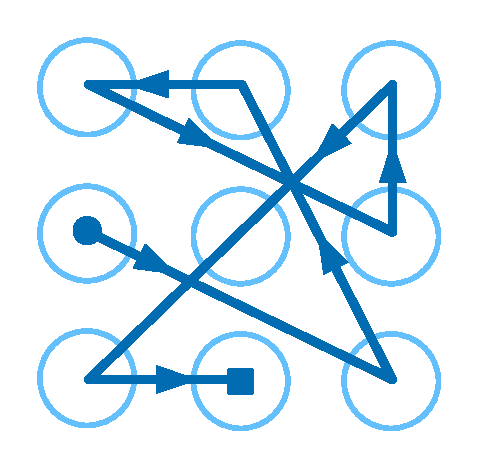
\includegraphics[width=1.3cm]{fig/9-12.pdf}
                \hspace{0.1cm}
                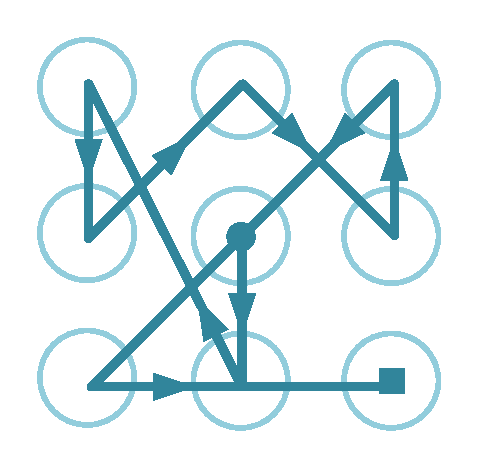
\includegraphics[width=1.3cm]{fig/9-13.pdf}
                \hspace{0.1cm}
                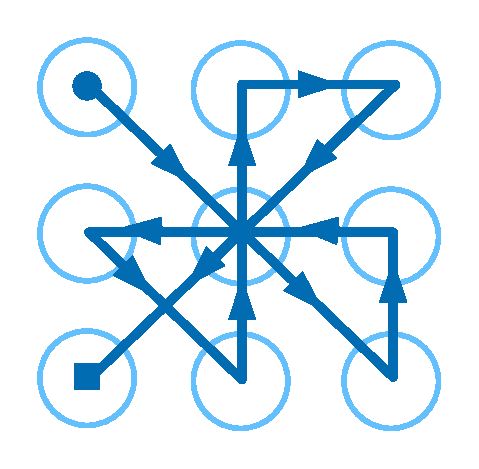
\includegraphics[width=1.3cm]{fig/9-14.pdf}
                \hspace{0.1cm}
                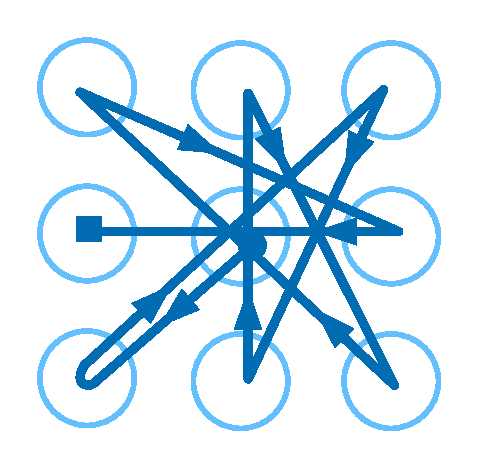
\includegraphics[width=1.3cm]{fig/9-15.pdf}\\
                \centering \footnotesize (c) Example patterns belong to the complex category.
                \end{minipage}
            }
            \caption{Examples of patterns collected from our participants. Patterns are grouped into \emph{simple}, \emph{median} and \emph{complex} categories, according to their complexity scores. }
            \label{fig:fig8}
            \vspace{-3mm}
        \end{figure}

        \begin{figure}[!t]
            \centering
            \subfigure{
                \begin{minipage}[b]{0.14\textwidth}
                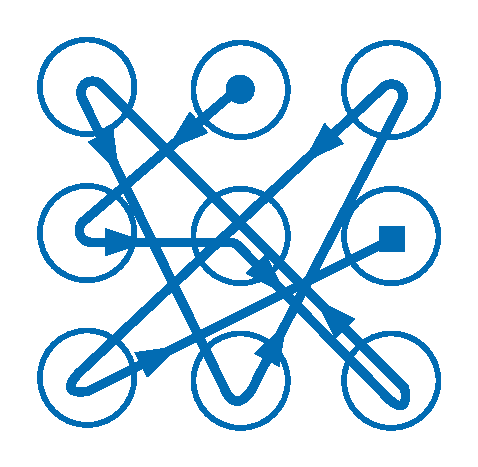
\includegraphics[width=0.8\textwidth]{fig/complex3.pdf} \\
                \centering \footnotesize complexity score: $43.8$
                \end{minipage}
            }
            \subfigure{
                \begin{minipage}[b]{0.14\textwidth}
                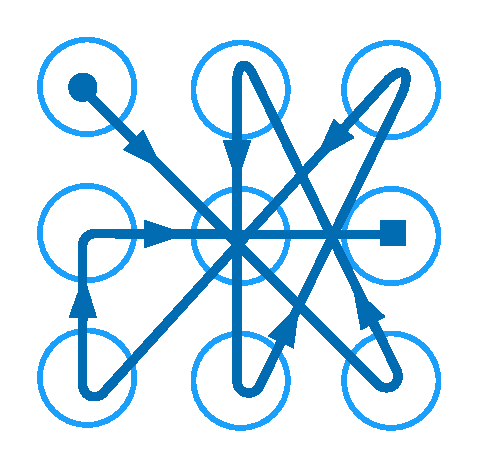
\includegraphics[width=0.8\textwidth]{fig/complex2.pdf} \\
                \centering \footnotesize complexity score: $44.7$
                \end{minipage}
            }
            \subfigure{
                \begin{minipage}[b]{0.14\textwidth}
                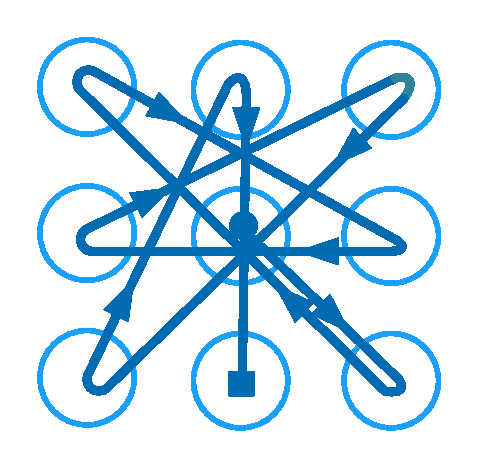
\includegraphics[width=0.8\textwidth]{fig/complex1.pdf} \\
                \centering \footnotesize complexity score: $46.8$
                \end{minipage}
            }
            \vspace{-2mm}
            \caption{Three most complex patterns on a $3\times 3$ grid based on Equation~\ref{equ:compscore}.}
            \vspace{-2mm}
            \label{fig:most complex patterns}
        \end{figure}

\section{Experimental Setup \label{sec:setup}}
    \subsection{Data Collection}
    \label{section:locking patterns}
    The patterns used in our evaluation were collected from users who use at least one Android device (a smartphone or a tablet) on a daily basis.
    To collect the patterns, we have distributed over 1,000 survey forms and collected back 215 valid forms, resulting in 120 unique patterns.
    Our participants include 95 females and 120 males who were undergraduate or postgraduate students in our institution.
    The majority of our participants are in an age group of under 30.


    To collect the patterns, we have conducted a ``pen-and-paper" survey by asking participants to fill in an anonymized questionnaire.
    The questionnaire and survey were approved by the research ethics board (REB) of our institution.
    We have made sure that our survey complied with strict privacy regulations. For example, we did not collect any personally identifiable information other than the gender and age group of the participant. Our participants were well informed on the purpose
    of the study and how the data will be managed and used. The survey forms were distributed as voluntary homework so that the participants can take the survey form away to fill in.
     Users were invited to return the survey form anonymously within three weeks to a dedicated, locked mailbox, if they wish to participate in the study.
     To avoid a user submits multiple copies of the same form, each survey form is given a unique, randomly generated 32-digital number.


     Overall, 37.6\% of our participants confirmed that they use pattern lock as the screen lock to
     protect their Android devices on a daily basis; and 33\% of those  who do not use a pattern as their screen lock said that they
     are often required to use a pattern for authentication by an application like \texttt{Alipay}. Furthermore, 60\%
     of our participants also indicated that the pattern they provided is currently being used
     or have been used in the past by themselves. Other participants (often those did not use a locking pattern on a daily basis) indicated that they
     have provided a pattern which they would like to use if a locking
     pattern is required. Based on this information, we are confident
     that our patterns represent some of the real world
     patterns. Finally, all participants believe that a complex pattern provides stronger protection than a simple one.


    \subsection{Pattern Complexity Classification}
    We quantify the complexity of a pattern using the complexity (strength) score proposed in~\cite{sun2014dissecting}.
        The complexity score, $CS_{P}$, of a pattern, $P$, is defined as:
    \begin{equation}
      CS_{P}=S_{P}\times\log_{2}(L_{P}+I_{P}+O_{P})
    \label{equ:compscore}
    \end{equation}
    where $S_{P}$ is the number of connected dots, $L_{P}$ is the the total length of all line segments that form the pattern (see Figure~\ref{fig:intersection-overlap}~a), $I_{P}$ are the number of intersections (which are also termed as ``knight moves" in some prior work~\cite{vonZezschwitz:2015:EDB:2702123.2702202}, see Figure~\ref{fig:intersection-overlap}~b) and $O_{P}$ are the number of overlapping linear segments (see Figure~\ref{fig:intersection-overlap}~c).  To calculate the line length, we assume the length between two horizontally or vertically adjunct dots is one. Thus, our method is independent of the size of the screen and the grid.


    Intuitively, the more connected dots ($S_{P}$), line segments ($L_{P}$),
    intersections ($I_{P}$) and overlapping line segments ($O_{P}$) that a
    pattern has, the more complex it is. For example, the patterns shown in
    Figure~\ref{fig:fig8} (c) use all the nine dots of the grid, and have  at
    least seven line segments and three intersections. %%However, we found


    Base on the complexity score, we divide the collected patterns into three complexity categories: \emph{simple}, \emph{median} and \emph{complex}. A simple pattern has a score of less than 19,
    a median
    complex pattern has a score between 19 and 33, and a complex pattern must have a score greater than 33. This classification gives us roughly 40 patterns per
    category. Figure~\ref{fig:fig8} gives some examples for each category while Figure~\ref{fig:pattern-strength} shows the distribution of these patterns according to their complexity scores.
    Based on this definition, the most complex pattern on a $3 \times 3$ grid has a score of $46.8$ (see Figure~\ref{fig:most complex patterns}).  The complex scores of the patterns we collected range from $6.4$ to $46.8$.

        \begin{figure}[!t]
            \centering
            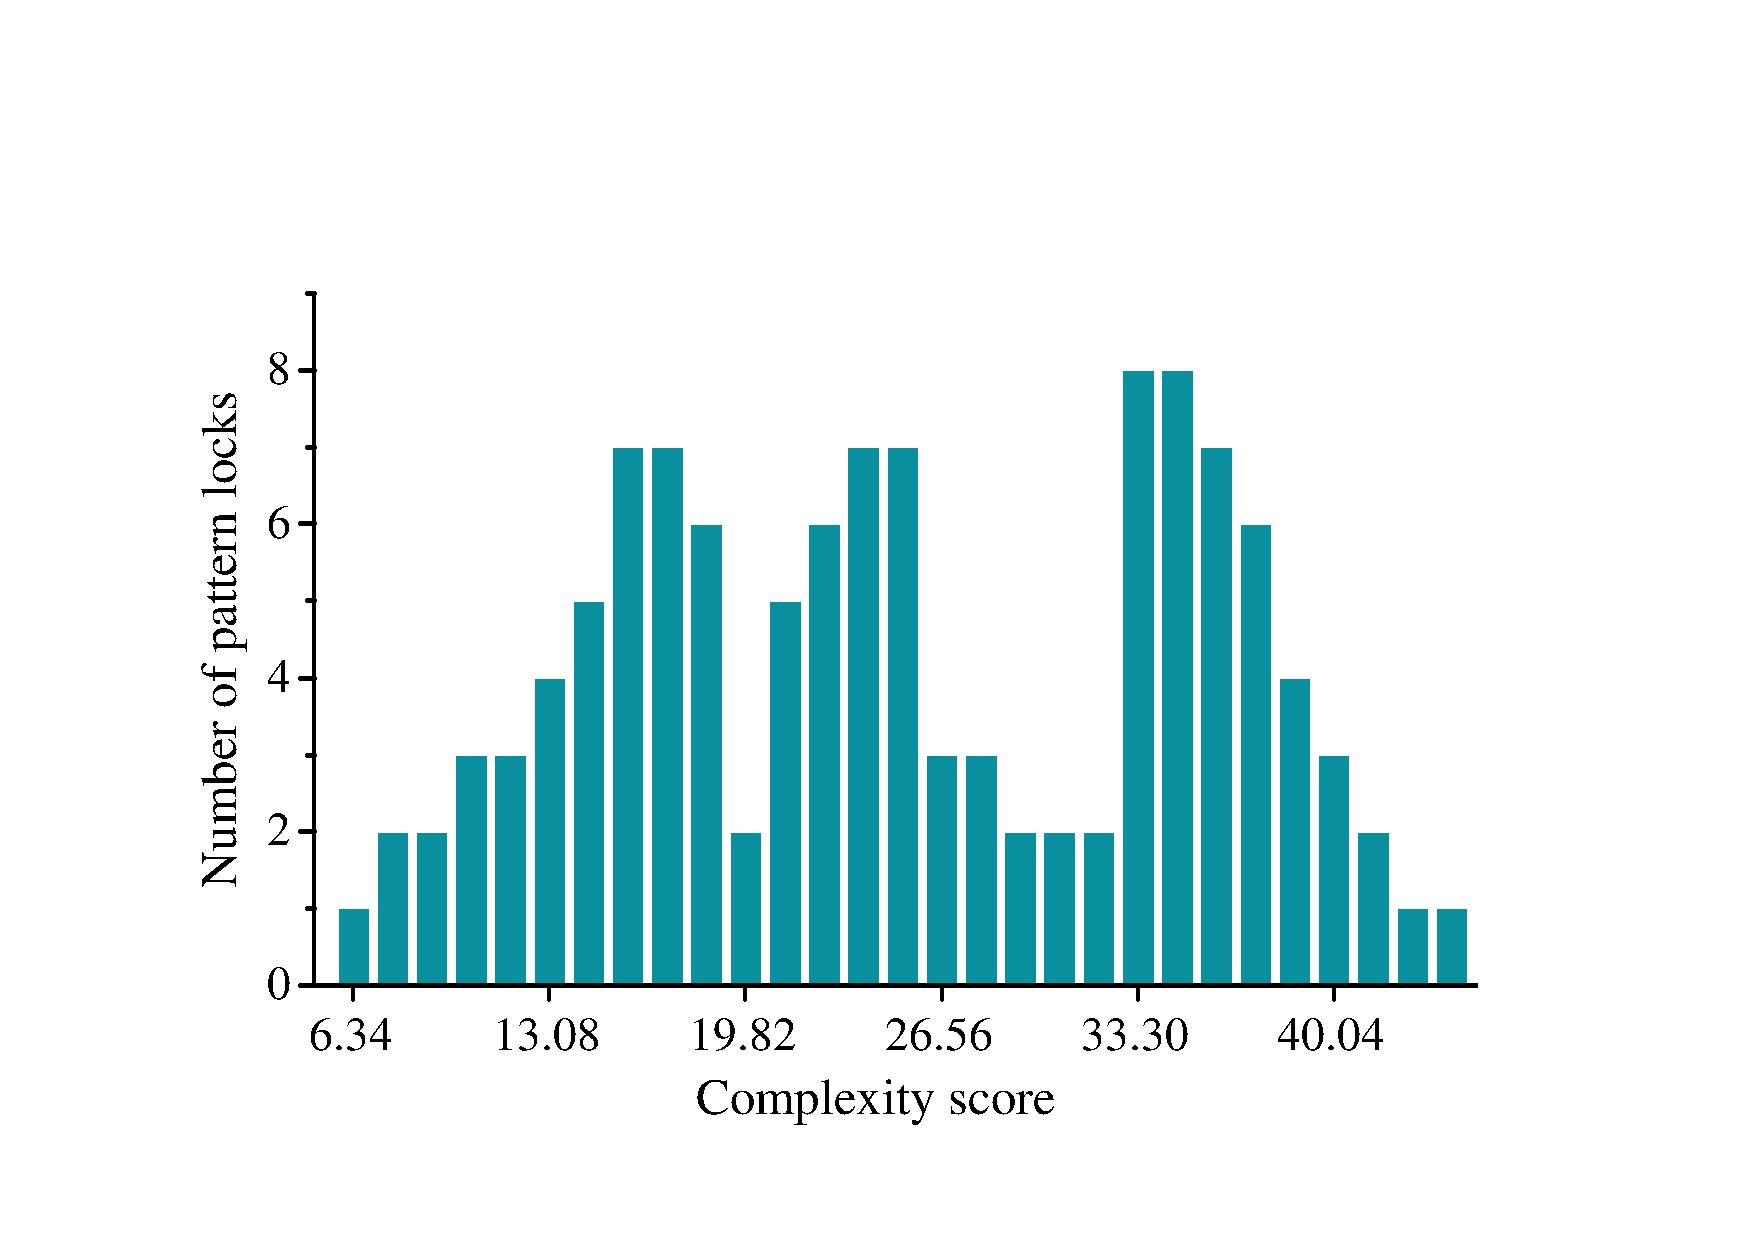
\includegraphics[width=0.35\textwidth]{fig/pattern-strength.pdf}
            \vspace{-3mm}
            \caption{The distribution of complexity scores for the patterns given by our participants.}
            \vspace{-2mm}
            \label{fig:pattern-strength}
        \end{figure}


    \begin{table}[!t]
            \centering
            \caption{Screen sizes for the test phones}
            \label{tab:locking-screen-size}
            \scriptsize
            \begin{tabular}{|c|c|c|c|}
                %\includegraphics[width=7.5cm]{fig/table1.pdf}
                \hline
                \diagbox[dir=SE]{Size}{Brands}& MI4 & Honor7 & Note4 \\
                \hline
                Height(cm)$\times$Width(cm) & $13.9\times6.9$ & $14.3\times7.2$ & $15.4\times7.9$ \\
                \hline
            \end{tabular}
            %\vspace{-4mm}
    \end{table}

    \subsection{Video Recording and Preprocessing}
    \noindent\textbf{Recording Devices} We used three smartphones for video recording: an Apple iPhone4S,
     a Xiaomi MI4 and a Meizu2 phones. Each mobile phone was used to record 40 patterns with a
    1080p HD resolution of 30 FPS under different settings.

    \noindent\textbf{User Participation} We recruited ten postgraduate students (five male and five female
    students) from our institution to reproduce the 120 patterns (collected from the users)
    and the 60 most complex patterns (see Section~\ref{sec:overall_rate})  on three target mobile phones:
    a Xiaomi MI4, a Huawei Honor7 and a Samsung Note4 smartphones. Table~\ref{tab:locking-screen-size} lists
    the screen size for each target mobile phone.


   \noindent\textbf{Video Recording Setup}
    By default, we used the  Android $3 \times 3$ native pattern grid,
    but we evaluated our approach using other pattern grids with different sizes in
    Section~\ref{sec:scalability}. We recorded each pattern under three filming
    angles, 45, 90 and 135 degrees, by placing the camera on the left-front, front, and right-front
    of the target device respectively.
    By default, the video
    was recorded indoor during daytime under a natural lighting condition. In
    Section~\ref{sec:light} we evaluated our approach under different lighting conditions
    both indoor and outdoor. By default, videos were recorded at a distance of
    2 meters from the target device and we evaluated the impact of the filming distance in
    Section~\ref{sec:scalability}.

    \noindent \textbf{Video Filming}
     Before recording, our participants were given the opportunity to practice a pattern
    several times, so that they can draw the pattern at
    their natural speed. On average, this practice session took 10 trails per user per pattern.
    When drawing the
    pattern, some participants sat, while others stood, some hold the device
    by hands, while others placed it on a table.
    Each pattern was drawn on three target devices and
    recorded under three filming angles. Thus, for the 120 patterns collected from users, we recorded 1,080 videos in total.

    \noindent\textbf{Video Preprocessing}
    For each video stream, we used the algorithm described in Section~\ref{sec:identify} to cut out the video segment
    of the unlocking process. We left around 200 to 300 milliseconds of the video segment before and after the pattern unlocking process.
    To track the fingertip locations,
    we used Windows Movie Make to highlight two areas of interest on the first frame of
    the video segment: one area surrounds the fingertip, and the other contains an edge of the
    phone (see Section~\ref {secction:shake}).

   \noindent\textbf{Implementation} Our prototyped attacking system built upon a TLD library~\cite{TLD-toolbox-web}.
    The developed software ran on an Intel Core i5 PC with
    8GB RAM. The operating system is Windows 10. Our implementation can be ported onto
    Android or Apple iOS systems, which is our future work. On our evaluation
    platform, our software takes less than 30 seconds to process a video to produce candidate patterns.
